\documentclass{amsart}
\usepackage{tikz}
\usepackage{tikz-cd}
\usepackage{tkz-graph}
\usetikzlibrary{arrows} 
\begin{document}
\begin{center}
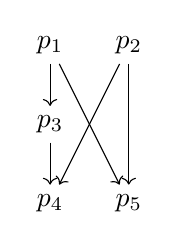
\begin{tikzpicture}
    \node (p1) at ( 0, 0) {$p_1$}; 
    \node (p2) at ( 1, 0) {$p_2$};
    \node (p3) at ( 0,-1) {$p_3$};
    \node (p4) at ( 0,-2) {$p_4$};
    \node (p5) at ( 1,-2) {$p_5$};

    \begin{scope}[every path/.style={->}]
       \draw (p1) -- (p3);
       \draw (p3) -- (p4); 
       \draw (p1) -- (p5);
       \draw (p2) -- (p4);
       \draw (p2) -- (p5);
    \end{scope}  
\end{tikzpicture}
\end{center}
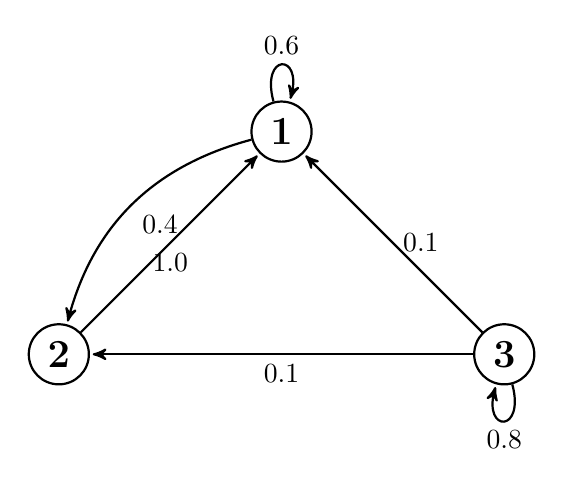
\begin{tikzpicture}[->,>=stealth',shorten >=1pt,auto,node distance=4cm,
                thick,main node/.style={circle,draw,font=\Large\bfseries}]

  \node[main node] (1) {1};
  \node[main node] (2) [below left of=1] {2};
  \node[main node] (3) [below right of=1] {3};

  \path
    (1) edge [loop above] node {0.6} (1)
        edge [bend right] node {0.4} (2)
    (2) edge node [below]{1.0} (1)
    (3) edge [loop below] node {0.8} (3)
        edge node[right] {0.1} (1)
        edge node[below] {0.1} (2);      
\end{tikzpicture}
\[
\begin{tikzcd} 
                                                                            &F_{4}=G_{4} \arrow{dr} \arrow{dl} \arrow{d} \\
\triangle_{3,1}(F_{4})=\triangle_{3,1}(G_{4}) \arrow{d} \arrow{dr}          &\triangle_{2,2}(F_{4})=\triangle_{2,2}(G_{4})    \arrow{dl} \arrow{dr}     \arrow{d}        &\triangle_{1,3}(F_{4})=\triangle_{1,3}(G_{4}) \arrow{d} \arrow{dl}\\
\triangle_{2,1,1}(F_{4})=\triangle_{2,1,1}(G_{4})  \arrow{dr}               & \triangle_{1,2,1}(F_{4})=\triangle_{1,2,1}(G_{4})         \arrow{d}                        & \triangle_{1,1,2}(F_{4})=\triangle_{1,1,2}(G_{4}) \arrow{dl}\\
                                                                            & \triangle_{1,1,1,1}(F_{4})=\triangle_{1,1,1,1}(G_{4})
\end{tikzcd}
\]
\end{document}